
\section{分离性与簇}

\textbf{11.2.1.\ \trhProposition{}。}\ ——\ \emph{设 $\pi\colon X\to Y$ 是概形之间的一个\trMorphism。}\\
\emph{(a) 若 $X$ 与 $Y$ 都是仿射的，那么\trDiagonalMorphism{} $\delta_\pi\colon X\to X\times_Y X$ 是一个\trClosedEmbedding。}\\
\emph{(b) 在一般情形，\trDiagonalMorphism{} $\delta_\pi\colon X\to X\times_Y X$ 是一个\trLocallyClosedEmbedding。}

$X\times_Y X$ 中与之相应的局部闭子概形——即\textbf{对角（局部闭）子概形}（diagonal (locally closed) subscheme）——将记作 $\Delta$。

\emph{证明。}\ （a）设 $X=\Spec A$，$Y=\Spec B$。于是\trDiagonalMorphism{}对应于自然的环映射 $A\otimes_B A\to A$，即由 $a_1\otimes a_2\mapsto a_1a_2$ 给出的那个映射，它显然是满射。

（b）我们将描述 $X\times_Y X$ 的一族\trOpenSubset{}，取其并来盖住 $X$ 的像，使得 $X$ 的像在这个并中是一个\trClosedEmbedding。

设 $Y$ 被\trAffine\trOpenSet{} $\mathsf{V}_i$ 所覆盖，而 $X$ 被\trAffine\trOpenSet{} $\mathsf{U}_{ij}$ 所覆盖，且 $\pi\colon\mathsf{U}_{ij}\to\mathsf{V}_i$。注意 $\mathsf{U}_{ij}\times_{\mathsf{V}_i}\mathsf{U}_{ij}$ 是积 $X\times_Y X$ 的一个\trAffine\trOpenSubscheme（我们当初构造积，基本上就是把仿射积木块粘合起来）。于是对角线被这些\trAffine\trOpenSubset{} $\mathsf{U}_{ij}\times_{\mathsf{V}_i}\mathsf{U}_{ij}$ 所覆盖。（$X$ 的任一点 $p$ 都落在某个 $\mathsf{U}_{ij}$ 中；于是 $\delta(p)\in\mathsf{U}_{ij}\times_{\mathsf{V}_i}\mathsf{U}_{ij}$。图~\ref{fig:diagonal-neighborhood} 或许有帮助。）注意 $\delta^{-1}(\mathsf{U}_{ij}\times_{\mathsf{V}_i}\mathsf{U}_{ij})=\mathsf{U}_{ij}$：一方面 $\mathsf{U}_{ij}\subset\delta^{-1}(\mathsf{U}_{ij}\times_{\mathsf{V}_i}\mathsf{U}_{ij})$ 是显然的；另一方面，由于 $\mathrm{pr}_1\circ\delta=\id_X$（其中 $\mathrm{pr}_1$ 是第一个\trProjection），又有 $\delta^{-1}(\mathsf{U}_{ij}\times_{\mathsf{V}_i}\mathsf{U}_{ij})\subset\mathsf{U}_{ij}$。最后，由 (a)，$\mathsf{U}_{ij}\to\mathsf{U}_{ij}\times_{\mathsf{V}_i}\mathsf{U}_{ij}$ 是一个\trClosedEmbedding。\hfill$\square$

\begin{figure}[htbp]
\centering
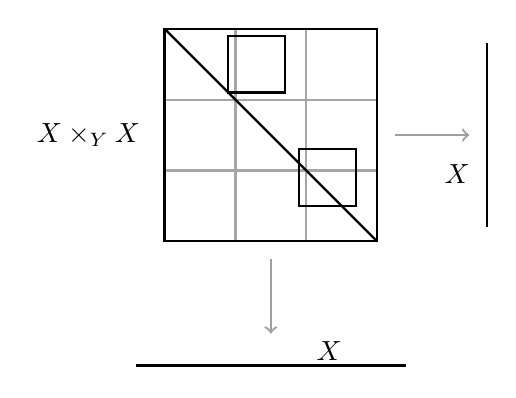
\begin{tikzpicture}[scale=0.9,line width=0.8pt]
  \draw[gray!70] (1,0) -- (1,3);
  \draw[gray!70] (2,0) -- (2,3);
  \draw[gray!70] (0,1) -- (3,1);
  \draw[gray!70] (0,2) -- (3,2);
  \draw (0,0) rectangle (3,3);
  \draw (0,3) -- (3,0);
  \draw (0.9,2.1) rectangle (1.7,2.9);
  \draw (1.9,0.5) rectangle (2.7,1.3);
  \node[anchor=east] at (-0.2,1.5) {$X\times_Y X$};
  \draw[gray!75,->] (3.25,1.5) -- (4.3,1.5);
  \draw (4.55,0.2) -- (4.55,2.8);
  \node[anchor=east] at (4.45,0.95) {$X$};
  \draw[gray!75,->] (1.5,-0.25) -- (1.5,-1.3);
  \draw (-0.4,-1.75) -- (3.4,-1.75);
  \node[anchor=west] at (2.0,-1.55) {$X$};
\end{tikzpicture}
\caption{对角线的一个开邻域被 $\mathsf{U}_{ij}\times_{\mathsf{V}_i}\mathsf{U}_{ij}$ 所覆盖。（依原书手绘图重绘。）}\label{fig:diagonal-neighborhood}
\end{figure}

我们所描述的这些开子集未必盖住 $X\times_Y X$，所以我们并没有证明 $\delta$ 是一个\trClosedEmbedding。

\textbf{11.2.A.（容易的练习）}\quad 设 $X\to Y$ 与 $X\to Z$ 都是\trLocallyClosedEmbedding。证明：$X\to Y\times Z$ 是\trLocallyClosedEmbedding。提示：\mbox{练习~11.1.E}。

\textbf{11.2.2.}\ \emph{\trhDefinition{}。}\quad \trMorphism{} $\pi\colon X\to Y$ 称为\textbf{\trSeparated}的（separated），若\trDiagonalMorphism{} $\delta_\pi\colon X\to X\times_Y X$ 是一个\trClosedEmbedding。一个 $A$-\trScheme{} $X$ 称为\textbf{在 $A$ 上\trSeparated}（separated over $A$），若\trStructureMorphism{} $X\to\Spec A$ 是\trSeparated{}的。当人们说概形（而非\trMorphism{}）$X$ 是\trSeparated{}的，他们默认指的是某个「\trStructureMorphism」是\trSeparated{}的。例如，若他们在谈论 $A$-\trScheme，他们的意思是 $X$ 在 $A$ 上\trSeparated。

多亏命题~11.2.1(b)（以及「像为闭集的\trLocallyClosedEmbedding{}实际上就是\trClosedEmbedding」这一事实，\mbox{练习~9.2.B}），\trMorphism{}是\trSeparated{}的，当且仅当对角线 $\Delta$ 是一个\trClosedSubset——这是对对角线的一条纯拓扑条件。这不禁让人想起\trHausdorff{}的一条定义，见下一道练习。

\textbf{11.2.B.（练习，仅为寻求拓扑动机的读者而设）}\quad 证明：\trTopologicalSpace{} $X$ 是\trHausdorff{}的，当且仅当对角线是 $X\times X$ 的\trClosedSubset。（概形的\trSeparatedness{}之所以不给出\trHausdorff{}性——也就是说，任意两点 $x$ 与 $y$ 未必有不相交的开\trNeighborhood——是因为在概形的\trCategory{}中，拓扑空间 $X\times X$ 一般不是拓扑空间 $X$ 与其自身的\trProduct；见 \S10.1.2。\footnote{原书此处作（for any two open points），「open」当系衍词，径删。——译者注}）

\textbf{11.2.3.\ \trhProposition{}。}\ ——\ \emph{\trSeparated{}态射构成 \S8.1 意义下的一个「合理」类——它们对\trComposition{}与\trBaseChange{}保持\footnote{原书此处作（they are by preserved），当系「they are preserved」之误，径改。——译者注}，并且这个概念是对目标局部的。}

\emph{证明。}\ \trClosedEmbedding{}这个类在这个意义下是「合理」的（\mbox{练习~10.4.A}），故由定理~11.1.2，\trSeparated{}态射亦然。\hfill$\square$

\textbf{11.2.C.（练习）}\quad 证明：\trMonomorphism{}都是\trSeparated{}的。从而\trLocallyClosedEmbedding（特别地，\trOpenEmbedding{}与\trClosedEmbedding）都是\trSeparated{}的。

\textbf{11.2.D.（练习）}\quad 证明：\trSeparated{}态射都是\trQuasiSeparated{}的。（提示：\trClosedEmbedding{}都是仿射的，从而是\trQuasicompact{}的。）

\textbf{11.2.4.\ \trhProposition{}。}\ ——\ \emph{仿射态射都是\trSeparated{}的。特别地，有限态射都是\trSeparated{}的。}

\emph{证明。}\ 由命题~11.2.1(a)，仿射概形之间的每个\trMorphism{}都是\trSeparated{}的。\trSeparatedness{}这个概念是对目标局部的，故得证。\hfill$\square$

下面的许多道练习都会让你切身体会到\trCancellationTheorem~11.1.1 的重要性。

\textbf{11.2.E.（练习）}\quad 证明：一个 $A$-\trScheme{}是\trSeparated{}的（在 $A$ 上），当且仅当它在 $\mathbb{Z}$ 上\trSeparated。特别地，一个复概形在 $\mathbb{C}$ 上\trSeparated，当且仅当它在 $\mathbb{Z}$ 上\trSeparated，所以复几何学家与算术几何学家可以毫无混淆地互谈\trSeparated{}概形。

\textbf{11.2.F.（容易的练习）}\quad 设有态射 $X\xrightarrow{\ \pi\ }Y\xrightarrow{\ \rho\ }Z$。\\
(a) 证明：若 $\rho\circ\pi$ 是\trLocallyClosedEmbedding（相应地，\trLocally\trFiniteType、\trSeparated），则 $\pi$ 亦然。\\
(b) 若 $\rho\circ\pi$ 是\trQuasicompact{}的，而 $Y$ 是\trNoetherian{}的，证明 $\pi$ 是\trQuasicompact{}的。提示：\cref{ex:quasicompact-quasiseparated-source}(a)。\\
(c) 若 $\rho\circ\pi$ 是\trQuasiSeparated{}的，证明 $\pi$ 是\trQuasiSeparated{}的。提示：\cref{ex:quasicompact-quasiseparated-source}(b)。

\textbf{11.2.G.（练习）}\quad 设 $\mu\colon Z\to X$ 是一个\trMorphism，而 $\sigma\colon X\to Z$ 是 $\mu$ 的一个\trSection，即 $\mu\circ\sigma$ 是 $X$ 上的恒等。
\[
\begin{tikzcd}[row sep=3.2em]
Z \ar[dd, "\mu", bend right=16] \\
& \\
X \ar[uu, "\sigma"', bend right=16]
\end{tikzcd}
\]
证明：$\sigma$ 是一个\trLocallyClosedEmbedding。证明：若 $\mu$ 是\trSeparated{}的，则 $\sigma$ 是一个\trClosedEmbedding。证明：若 $\mu$ 是\trQuasiSeparated{}的，则 $\sigma$ 是\trQuasicompact{}的。举出一个例子，说明当 $\mu$ 不\trSeparated{}时，$\sigma$ 未必是\trClosedEmbedding。

\textbf{11.2.5.}\ \emph{\trGraphMorphism{}。}\quad 设 $\pi\colon X\to Y$ 是 $Z$-\trScheme{}之间的一个\trMorphism。由 $\gamma_\pi=(\id,\pi)$ 给出的\trMorphism{} $\gamma_\pi\colon X\to X\times_Z Y$ 称为\textbf{\trGraphMorphism{}}（graph morphism）（见图~\ref{fig:graph-morphism}）。（它曾秘密地出现在\mbox{练习~11.1.A}中。）于是 $\pi$ 可分解为 $\mathrm{pr}_2\circ\gamma_\pi$，其中 $\mathrm{pr}_2$ 是第二个\trProjection。图~\ref{fig:graph-morphism} 中的方图常被称为\textbf{态射 $\pi$ 的图像}（graph）。（我们将在 \S11.3.4 中讨论有理映射的图像。）把\mbox{练习~11.2.G}应用到 $X\times_Z Y\to X$ 上，便得到：

\begin{figure}[htbp]
\centering
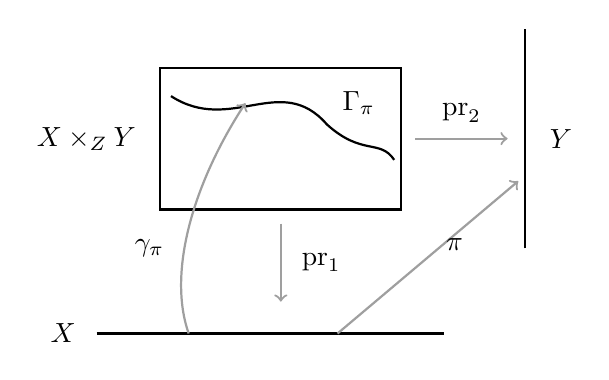
\begin{tikzpicture}[scale=0.9,line width=0.8pt]
  \draw (0,0) rectangle (3.4,2.0);
  \draw (0.15,1.6) .. controls (1.0,1.05) and (1.7,1.95) .. (2.35,1.2)
        .. controls (2.85,0.75) and (3.1,1.0) .. (3.3,0.7);
  \node at (2.8,1.5) {$\Gamma_\pi$};
  \node[anchor=east] at (-0.2,1.0) {$X\times_Z Y$};
  \draw[gray!75,->] (3.6,1.0) -- (4.9,1.0);
  \node[anchor=south] at (4.25,1.08) {$\mathrm{pr}_2$};
  \draw (5.15,-0.55) -- (5.15,2.55);
  \node[anchor=west] at (5.35,1.0) {$Y$};
  \draw[gray!75,->] (1.7,-0.2) -- (1.7,-1.3);
  \node[anchor=west] at (1.85,-0.75) {$\mathrm{pr}_1$};
  \draw (-0.9,-1.75) -- (4.0,-1.75);
  \node[anchor=east] at (-1.05,-1.75) {$X$};
  \draw[gray!75,->] (0.4,-1.75) .. controls (0.1,-0.9) and (0.45,0.35) .. (1.2,1.5);
  \node[anchor=east] at (0.2,-0.55) {$\gamma_\pi$};
  \draw[gray!75,->] (2.5,-1.75) -- (5.05,0.4);
  \node at (4.15,-0.5) {$\pi$};
\end{tikzpicture}
\caption{\trGraphMorphism{}。（依原书手绘图重绘。）}\label{fig:graph-morphism}
\end{figure}

\textbf{11.2.6.\ \trhProposition{}。}\ ——\ \emph{\trGraphMorphism{} $\gamma_\pi$ 总是一个\trLocallyClosedEmbedding。若 $Y$ 是\trSeparated{}的 $Z$-\trScheme（即 $Y\to Z$ 是\trSeparated{}的），则 $\gamma_\pi$ 是一个\trClosedEmbedding。若 $Y$ 是\trQuasiSeparated{}的 $Z$-\trScheme，则 $\gamma_\pi$ 是\trQuasicompact{}的。}

$\gamma_\pi$ 的像（$X\times_Z Y$ 的一个局部闭子概形）也常被称为 $\pi$ 的\textbf{图像}（graph of $\pi$）；我们可以把它记作 $\Gamma_\pi$。

\textbf{11.2.H.（我们不会用到的练习）}\quad 设 $P$ 是一个\trMorphism{}类：\trClosedEmbedding{}都在 $P$ 中，且 $P$ 对\trFiberProduct{}与\trComposition{}保持。回想关于态射「\trReduction」的定义~10.7.8。证明：若 $\pi\colon X\to Y$ 属于 $P$，则 $\pi^{\mathrm{red}}\colon X^{\mathrm{red}}\to Y^{\mathrm{red}}$ 属于 $P$。（两个例子是\trSeparated{}态射类与\trQuasiSeparated{}态射类。）可能的提示：
\[
\begin{tikzcd}[row sep=2.6em, column sep=3.4em]
X^{\mathrm{red}} \ar[r, "\pi^{\mathrm{red}}"] \ar[d, "\in P"'] \ar[dr] &
Y^{\mathrm{red}} \ar[d, "\in P\delta"] \\
X \ar[r, "\pi\in P"'] & Y.
\end{tikzcd}
\]

\textbf{11.2.7.\ 重要的例子。}

\textbf{11.2.I.（练习）}\quad 证明：原点加倍了的\trAffineLine（例~4.4.5）不是\trSeparated{}的，办法是验证\trDiagonalMorphism{}的像不是\trClosedSubset。（下文的\mbox{练习~11.3.C}给出另一个论证；\mbox{练习~13.7.C}将给出一个花哨的论证。）

我们马上迎来第一个「\trSeparated{}但不仿射」的例子。下面这区区一步计算就将蕴涵：所有拟射影 $A$-\trScheme{}都是\trSeparated{}的（一旦我们知道\trSeparated{}态射的\trComposition{}仍是\trSeparated{}的，命题~11.2.3）。

\textbf{11.2.8.\ \trhProposition{}。}\ ——\ \emph{态射 $\mathbb{P}^n_A\to\Spec A$ 是\trSeparated{}的。}

我们给出两个证明。第一个靠直接计算；第二个无须任何计算，只要求你记得前面讲过的一些经典构造。

\emph{证明~1：直接计算。}\ 我们用形如 $\mathsf{U}_i\times_A\mathsf{U}_j$ 的开集覆盖 $\mathbb{P}^n_A\times_A\mathbb{P}^n_A$，其中 $\mathsf{U}_0,\dots,\mathsf{U}_n$ 构成「通常的」\trAffine\trOpenCover。$i=j$ 的情形此前已在命题~11.2.1(a) 的证明中处理过。若 $i\neq j$，则
\[
\mathsf{U}_i\times_A\mathsf{U}_j\cong\Spec A[x_{0/i},\dots,x_{n/i},\,y_{0/j},\dots,y_{n/j}]/(x_{i/i}-1,\ y_{j/j}-1).
\]
现在 $\delta^{-1}(\mathrm{pr}_1^{-1}(\mathsf{U}_i))$ 就是 $\mathsf{U}_i$（因为\trDiagonalMorphism{}与到第一个因子的\trProjection{}复合是恒等映射），类似地 $\mathsf{U}_j=\delta^{-1}(\mathrm{pr}_2^{-1}(\mathsf{U}_j))$。于是 $\delta^{-1}(\mathsf{U}_i\times_A\mathsf{U}_j)=\mathsf{U}_i\cap\mathsf{U}_j$，所以在 $\mathsf{U}_i\times_A\mathsf{U}_j$ 上的\trDiagonalMorphism{}就是 $\mathsf{U}_i\cap\mathsf{U}_j\to\mathsf{U}_i\times_A\mathsf{U}_j$。这是一个\trClosedEmbedding，因为相应的环映射
\[
A[x_{0/i},\dots,x_{n/i},y_{0/j},\dots,y_{n/j}]
\longrightarrow
A[x_{0/i},\dots,x_{n/i},x_{j/i}^{-1}]/(x_{i/i}-1)
\]
（由 $x_{k/i}\mapsto x_{k/i}$、$y_{k/j}\mapsto x_{k/i}/x_{j/i}$ 给出）显然是满射（右边的环的每个生成元都显然落在像中——注意 $x_{j/i}^{-1}$ 是 $y_{i/j}$ 的像）。\hfill$\square$

\emph{证明~2：经典几何。}\ 注意：\trDiagonalMorphism{} $\delta\colon\mathbb{P}^n_A\to\mathbb{P}^n_A\times_A\mathbb{P}^n_A$ 复合上 \trSegre{}嵌入 $S\colon\mathbb{P}^n_A\times_A\mathbb{P}^n_A\to\mathbb{P}^{n^2+2n}$（\S10.6，一个\trClosedEmbedding）之后，也可以分解为第二个\trVeroneseEmbedding{} $v_2\colon\mathbb{P}^n_A\to\mathbb{P}^{\binom{n+2}{2}-1}$（\S9.3.6）与一个线性映射 $L\colon\mathbb{P}^{\binom{n+2}{2}-1}\to\mathbb{P}^{n^2+2n}$ 的复合，而这两者都是\trClosedEmbedding（线性映射 $L$ 的情形由\mbox{练习~9.3.C}给出）。
\[
\begin{tikzcd}[row sep=2.9em, column sep=3.4em]
& \mathbb{P}^n_A\times_A\mathbb{P}^n_A
  \ar[dl, "\delta", "\text{局部（？）闭嵌入}"'] \ar[dr, "S", "\text{闭嵌入}"'] & \\
\mathbb{P}^n_A \ar[dr, "v_2"', "\text{闭嵌入}"'] & & \mathbb{P}^{n^2+2n} \\
& \mathbb{P}^{\binom{n+2}{2}-1} \ar[ur, "L"', "\text{闭嵌入}"'] &
\end{tikzcd}
\]
不严格地说，用坐标来看：
{\small
\[
\begin{tikzcd}[row sep=3.2em, column sep=2.2em]
& \bigl([x_0,x_1,\dots,x_n],\,[x_0,x_1,\dots,x_n]\bigr)
  \ar[dl, "\delta"'] \ar[dr, "S"] & \\
{[x_0,x_1,\dots,x_n]} \ar[dr, "v_2"'] & &
{\begin{bmatrix}
x_0^2 & x_0x_1 & \cdots & x_0x_n \\
x_1x_0 & x_1^2 & \cdots & x_1x_n \\
\vdots & \vdots & \ddots & \vdots \\
x_nx_0 & x_nx_1 & \cdots & x_n^2
\end{bmatrix}} \\
& {[x_0^2,x_0x_1,\dots,x_{n-1}x_n,x_n^2].} \ar[ur, "L"'] &
\end{tikzcd}
\]
}
复合映射 $\mathbb{P}^n_A\to\mathbb{P}^{n^2+2n}$ 可以写成
\[
[x_0,\dots,x_n]\mapsto[x_0^2,\,x_0x_1,\,x_0x_2,\,\dots,\,x_n^2],
\]
其中右边的下标跑遍一切满足 $0\le i,j\le n$ 的有序对 $(i,j)$。这就迫使 $\delta$ 把闭集送到闭集（否则 $S\circ\delta$ 就不会如此，而 $L\circ v_2$ 会）。\hfill$\square$

\textbf{11.2.9.\ 重要的定义（终于！）。}\quad 域 $k$ 上的一个\textbf{\trVariety}（variety），或称 \textbf{$k$-\trVariety}（$k$-variety），是 $k$ 上一个既约、\trSeparated{}的有限型概形。例如，既约的有限型仿射 $k$-\trScheme{}就是一个\trVariety。（你看出\trSeparatedness{}为何成立了吗？）\trVariety{}这个观念推广了我们早先的仿射簇（\S5.3.7）与射影簇（\S5.3.7；见推论~11.2.15）的观念。由\mbox{练习~5.3.F}，\trVariety{}的\trClosedPoint{}是\trDense{}的。（记号警示：在另一些文献里，还会附加\trIrreducibility{}这条条件；此外也常假定 $k$ 是\trAlgClosedField。）

$k$ 上的\trVariety{}构成一个\trCategory{}：$k$-\trVariety{}之间的\trMorphism{}就是作为 $k$-\trScheme{}的\trMorphism{}。（当然，代数闭域 $k$ 上的\trVariety{}的\trCategory{}，远在现代\trSchemeTheory{}之前就早已存在。）

\textbf{11.2.J.（容易的练习）}\quad 证明：$k$-\trVariety{}之间的\trMorphism{}都是有限型的，并且是\trSeparated{}的。

\trVariety{} $X$ 的一个\textbf{\trSubvariety{}}（subvariety）是 $X$ 的一个\emph{既约}局部闭子概形（你可以很快验证：它本身就是\trVariety）。$X$ 的开\trSubvariety{}是 $X$ 的一个\trOpenSubscheme（此时既约性是自动的）。$X$ 的闭\trSubvariety{}是 $X$ 的一个既约\trClosedSubscheme。

\textbf{11.2.K.}\ \extrahard\ \textbf{（练习，面向背景合适的读者：复代数簇给出复解析簇）}\quad 证明：复代数簇的\trAnalytification{}（\mbox{练习~7.3.P}）是一个复解析簇。

\textbf{11.2.10.\ \trVariety{}的\trProduct{}。}

\textbf{11.2.11.\ \trhProposition{}。}\ ——\ \emph{(a) 若 $k$ 是\trPerfectField，则 $k$-\trVariety{}的\trProduct（$\Spec k$ 上的\trFiberProduct）是一个 $k$-\trVariety。}\\
\emph{(b) 若 $k$ 是\trAlgClosedField，则不可约 $k$-\trVariety{}的\trProduct{}是一个不可约 $k$-\trVariety。}\\
\emph{(c) 若 $k$ 是\trAlgClosedField，则连通 $k$-\trVariety{}的\trProduct{}是一个连通 $k$-\trVariety。}

\emph{证明。}\ (a) 有限型与\trSeparated{}这两条陈述是直截了当的，因为这两条性质都对\trBaseChange{}与\trComposition{}保持。至于既约性：先化归到仿射情形，再用推论~10.5.23。

(b) 只剩下证明不可约性。用\mbox{练习~10.5.N}化归到仿射情形（如命题~10.5.15 的证明那样），再用\mbox{练习~10.5.M}，后者需要可分闭包。（作为练习，你可以改用\mbox{练习~10.4.H}，从而避开 \S10.5 的种种繁难。）

\textbf{11.2.L.（练习）}\quad 证明 (c)。\hfill$\square$

\textbf{11.2.12.\ 回到\trSeparatedness{}。}\quad 这里是\trSeparatedness{}的一条非常顺手的推论。

\textbf{11.2.13.\ \trhProposition{}。}\ ——\ \emph{设 $X\to\Spec A$ 是向一个\trAffineScheme{}的\trSeparated{}态射，而 $\mathsf{U}$ 与 $\mathsf{V}$ 是 $X$ 的\trAffine\trOpenSubset。那么 $\mathsf{U}\cap\mathsf{V}$ 是 $X$ 的一个仿射开子集。}

在证明之前，先给出一条出人意料的推论。取 $X=\Spec A$，我们便看到：$\Spec A$ 的任意两个仿射开子集的交也是仿射开子集。这一点当然绝不显然！我们知道两个特异仿射开子集的交是仿射的（由 $D(f)\cap D(g)=D(fg)$），但对一般的仿射开子集，我们几乎束手无策。

\trhWarning{}：这条性质并不刻画\trSeparatedness{}。（正确的性质是「\trAffineDiagonal{}」（affine-diagonal），我们将不讨论它，但它在\trStack{}理论中很有用。）例如，若 $A$ 是域 $k$，而 $X$ 是 $k$ 上原点加倍了的\trAffineLine，则 $X$ 也具有这条性质。

在命题~11.2.13 的证明中，我们将用到下面这个漂亮的结果。

\textbf{11.2.M.（容易的练习）}\quad 设 $\mathsf{U}$ 与 $\mathsf{V}$ 是 $A$-\trScheme{} $X$ 的\trOpenSubset。证明：$\mathsf{U}\cap(\mathsf{U}\times_A\mathsf{V})\cong\mathsf{U}\cap\mathsf{V}$。（两个局部闭子概形的交，其定义见\cref{ex:intersection-locally-closed-embeddings}。）提示：(i) 这在命题~11.2.8 的证明~1 的过程中已被基本证明。(ii) 见图~\ref{fig:diagonal-intersection}。(iii) 你可以用对角—基变换图（\cref{ex:diagonal-base-change-square}）来解读这条陈述：
\[
\begin{tikzcd}[row sep=2.4em, column sep=3.2em]
\mathsf{U}\cap\mathsf{V} \ar[r] \ar[d] & \mathsf{U}\times_A\mathsf{V} \ar[d] \\
X \ar[r, "\delta"'] & X\times_A X.
\end{tikzcd}
\]

\begin{figure}[htbp]
\centering
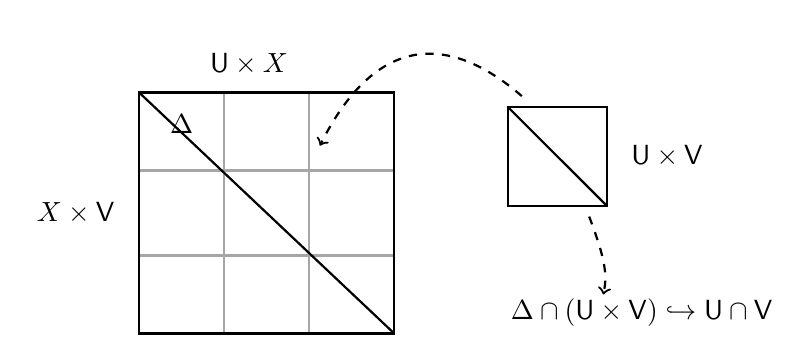
\begin{tikzpicture}[scale=0.9,line width=0.8pt]
  \draw[gray!70] (1.2,0) -- (1.2,3.4);
  \draw[gray!70] (2.4,0) -- (2.4,3.4);
  \draw[gray!70] (0,1.1) -- (3.6,1.1);
  \draw[gray!70] (0,2.3) -- (3.6,2.3);
  \draw (0,0) rectangle (3.6,3.4);
  \draw (0,3.4) -- (3.6,0);
  \node at (0.6,2.95) {$\Delta$};
  \node[anchor=south] at (1.55,3.5) {$\mathsf{U}\times X$};
  \node[anchor=east] at (-0.2,1.7) {$X\times\mathsf{V}$};
  \draw (5.2,1.8) rectangle (6.6,3.2);
  \draw (5.2,3.2) -- (6.6,1.8);
  \node[anchor=west] at (6.8,2.5) {$\mathsf{U}\times\mathsf{V}$};
  \draw[dashed,->] (5.4,3.35) .. controls (4.3,4.3) and (3.3,4.15) .. (2.55,2.65);
  \draw[dashed,->] (6.35,1.65) .. controls (6.6,1.0) and (6.6,0.8) .. (6.55,0.55);
  \node[anchor=west] at (5.1,0.3) {$\Delta\cap(\mathsf{U}\times\mathsf{V})\hookrightarrow\mathsf{U}\cap\mathsf{V}$};
\end{tikzpicture}
\caption{$\Delta\cap(\mathsf{U}\times\mathsf{V})\cong\mathsf{U}\cap\mathsf{V}$（\mbox{练习~11.2.M}）。（依原书手绘图重绘。）}\label{fig:diagonal-intersection}
\end{figure}

\textbf{11.2.14.}\ \emph{命题~11.2.13 的证明。}\quad 由\mbox{练习~11.2.M}，$(\mathsf{U}\times_A\mathsf{V})\cap\Delta\cong\mathsf{U}\cap\mathsf{V}$，其中 $\Delta$ 是对角线。但 $\mathsf{U}\times_A\mathsf{V}$ 是仿射的（两个仿射概形在仿射概形上的\trFiberProduct{}是仿射的：见我们构造纤维积的第 1 步，定理~10.1.1），而 $(\mathsf{U}\times_A\mathsf{V})\cap\Delta$ 是仿射概形 $\mathsf{U}\times_A\mathsf{V}$ 的一个\trClosedSubscheme，从而 $\mathsf{U}\cap\mathsf{V}$ 是仿射的。\hfill$\square$

\textbf{11.2.15.\ \trhCorollary{}。}\ ——\ \emph{每个拟射影 $A$-\trScheme{}都在 $A$ 上\trSeparated。特别地，每个既约的拟射影 $k$-\trScheme{}都是一个 $k$-\trVariety。}

\emph{证明。}\ 设 $X\to\Spec A$ 是一个拟射影 $A$-\trScheme。\trStructureMorphism{}可以分解为一个\trOpenEmbedding{}复合一个\trClosedEmbedding{}再复合 $\mathbb{P}^n_A\to\Spec A$。\trOpenEmbedding{}与\trClosedEmbedding{}都是\trSeparated{}的（\mbox{练习~11.2.C}），而 $\mathbb{P}^n_A\to\Spec A$ 是\trSeparated{}的（命题~11.2.8）。\trSeparated{}态射的\trComposition{}仍是\trSeparated{}的（命题~11.2.3），故得证。\hfill$\square$

下面是一道我们用不上、但你或许会喜欢的练习。它包含命题~11.2.13 的一个逆命题。

\textbf{11.2.N.（练习）}\quad 证明：$X\to\Spec A$ 是\trSeparated{}的，当且仅当对 $X$ 的所有\trAffine\trOpenSubset{} $\mathsf{U}$ 与 $\mathsf{V}$：(i) 交 $\mathsf{U}\cap\mathsf{V}$ 是仿射的，(ii) 映射 $\OO(\mathsf{U})\otimes_A\OO(\mathsf{V})\to\OO(\mathsf{U}\cap\mathsf{V})$ 是满射。证明：当 $\mathsf{U}$ 与 $\mathsf{V}$ 取遍任一\trAffine\trCover{} $X=\bigcup\mathsf{U}_i$ 中的集合时，检验上述两点就够了。（提示：命题~11.2.8 的证明~1 已把这件事做了大半。）

\textbf{11.2.16.}\ \extrahard\ \textbf{泛单射\trMorphism{}与对角线。}

\textbf{11.2.O.（练习）}\quad 证明：$\pi\colon X\to Y$ 是\textbf{\trUniversallyInjective}的（universally injective），当且仅当\trDiagonalMorphism{} $\delta_\pi\colon X\to X\times_Y X$ 是满态射。（回想：由命题~11.2.1(b)，$\delta_\pi$ \emph{总是}单的。）

由于满态射构成一个「合理」类（\mbox{练习~10.4.G}），我们看到泛单射态射也构成一个「合理」类。

\textbf{11.2.P.（容易的练习）}\quad 若 $\pi\colon X\to Y$ 与 $\rho\colon Y\to Z$ 是\trMorphism，而 $\rho\circ\pi$ 是泛单射的，证明 $\pi$ 是泛单射的。

\textbf{11.2.Q.（练习）}\\
(a) 证明：泛单射态射都是\trSeparated{}的。\\
(b) 证明：\trAlgClosedField{} $\overline{k}$ 上两个有限型概形之间的映射是泛单射的，当且仅当它在\trClosedPoint{}上是\trInjectiveMap。
